% e3march-user-guide.tex
% PJ, June 2014
%
\documentclass[12pt,a4paper,twoside]{article}
\usepackage[body={16cm,24.5cm}]{geometry}
\usepackage{hyperref}
\hypersetup{colorlinks=true,linkcolor=blue}
\usepackage{graphicx}
\usepackage{makeidx}
% \usepackage{showidx}
\usepackage{listings}
\usepackage{lscape}
\usepackage{longtable}
\usepackage{amsmath}
\usepackage{amssymb}
\usepackage{subfig}
\lstset{basicstyle=\ttfamily\scriptsize, showstringspaces=false, identifierstyle=, keywordstyle=}
\lstset{numbers=left, numberstyle=\tiny, stepnumber=1, numbersep=5pt}
\newcommand{\code}[2]{
 \hrulefill
 \scriptsize
 \lstinputlisting{#2}
 \hrulefill
 \vspace{2em}
 \normalsize
}
%\usepackage{booktabs}
%\usepackage{pgfplots} \pgfplotsset{compat=newest} % Doesn't work on LinuxMint 13; need something more recent.

%------------------------------------------------------------------
% a couple horizontal bars to delimit embedded code
% the width suits the page size set above and
% the mathmode eliminates spaces between the three elements
\newcommand{\topbar}{\ensuremath{
    \rule{0.1mm}{2.0mm} \rule[2.0mm]{159.5mm}{0.1mm} \rule{0.1mm}{2.0mm}
}}
\newcommand{\bottombar}{\ensuremath{
    \rule{0.1mm}{2.0mm} \rule{159.5mm}{0.1mm} \rule{0.1mm}{2.0mm}
}}
\newcommand{\topbarshort}{\ensuremath{
    \rule{0.1mm}{2.0mm} \rule[2.0mm]{149.5mm}{0.1mm} \rule{0.1mm}{2.0mm}
}}
\newcommand{\bottombarshort}{\ensuremath{
    \rule{0.1mm}{2.0mm} \rule{149.5mm}{0.1mm} \rule{0.1mm}{2.0mm}
}}
%------------------------------------------------------------------

\title{
    A block-marching {CFD} solver for compressible flow.
}
\author{
    Mechanical Engineering Report 2014/06\\
    Wilson Y. K. Chan ~ Peter A. Jacobs  ~ Fabian Zander\thanks{Institut fuer Raumfahrtsysteme
      Universitaet Stuttgart, Pfaffenwaldring 29, 70569 Stuttgart.}\\
    ~ Rowan J. Gollan and Luke Doherty\\
    Centre for Hypersonics, The University of Queensland, Brisbane, Australia.
}
\makeindex

\begin{document}
\maketitle

\begin{abstract}

\end{abstract}

\cleardoublepage
\tableofcontents

%------------------------------------------------------------------
\cleardoublepage
\baselineskip = 1.5pc

\section{Introduction}
%
Eilmer3 is a transient compressible flow solver that uses block-structured 
grids\,\cite{gollan_jacobs_2013a,jacobs_etal_2014a,jacobs_etal_2014b}.  
Since it is a simulation code that uses explicit updates for the solution 
of the full Navier-Stokes equations and all parts of the flow field are included in all time steps, 
the calculation can become very computationally expensive, especially when using fine grids.  
Further, if the primary interest is in the long-term or steady-state solution over the domain, 
much of the intermediate (transient flow) data is irrelevant and is then discarded.

\medskip
A large class of flow problems of interest to our research group may be described 
as mostly supersonic flow with a dominant direction and having duct-like boundary surfaces.  
Specific examples include supersonic wind-tunnel nozzles and scramjet inlets, combustors and thrust nozzles.  
For these flows, the upstream parts of the flow field settle early and remain unchanged 
while the downstream parts of the flow solution evolve to steady state.  
Of course, specialized CFD codes based on parabolized Navier-Stokes equations are available 
for producing fast solutions for this class of flow, however, 
they are limited in the presence of strong shock-wave boundary-layer interactions.

\medskip
The “block-marching” approach that we have developed for Eilmer3 has some advantages 
in that it retains the use of the full transient solver for 
the complete Navier-Stokes equations but accelerates the overall computation 
by concentrating on subsets of blocks, until they reach steady-state, 
marching in the dominant flow direction and building up the steady solution for the full domain. 
Our first attempt at making the flow simulation code into a form of space-marching code
was to sequence the processing of blocks within the main C++ sumulation code\,\cite{zander_etal_2011b},
however, that approach could not easily make use of many processors on a cluster computer. 
Instead, a higher-level \textit{coordinating} approach was coded 
as a set of shell scripts which coordinated separate computation jobs on subsets of blocks
and could make use of several processors by running these jobs on the local cluster computer\,\cite{chan_2012a}.  

\medskip
The present implementation has been rewritten in a modern scripting language (Python) 
and is essentially a coordinating program that delegates the actual work 
of solving the flow equations on subsets of the original grid to an underlying CFD solver.  
Behind the scenes, it generates a potentially large simulation, 
with many block-structured grids covering the full domain and organised in a regular array.  
It then works through the large array of blocks, one subset at a time, 
setting up a small transient calculation with adjusted boundary conditions and 
submitting that to the original transient solver for integration.  
On the completion of each sub-problem, the coordinating program marshalls the blocks 
of steady state data such that the full set of blocks is finally presented 
as a single solution field at the end of the process.  
A computational advantage of this approach is that we may continue to make use 
of a cluster computer to accelerate the individual subset calculations.  
As well, it requires no changes to the underlying flow solver, 
so it may be applied to any flow solver for which we can automate the writing of job files. 

\medskip
In the following sections, we will more completely describe the approach 
and provide verification and validation examples.  
% We will also provide an example of its application to nozzle flow calculation 
% and nozzle surface design, an application that benefits greatly 
% from having fast flow calculations available.


\section{Simulation Process -- Block Marching}
%
To aid the description of the block-marching approach, a simple example which involves 
Mach\,4 flow over a 10$^\circ$ wedge is used. The geometrical setup for this example is 
shown in Figure~\ref{f:10-deg-wedge-schema}. For this example, a total of eight blocks is 
used, and the direction of Mach\,4 inflow is from left to right.
%
\begin{figure}[htbp]
   \centerline{ 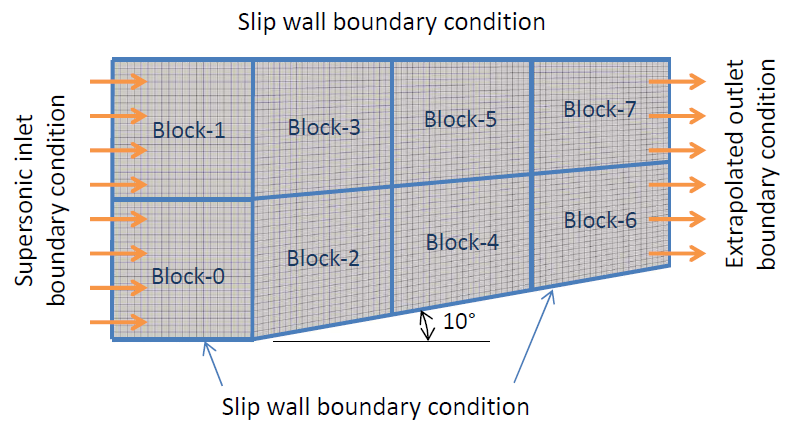
\includegraphics[width=10cm]{figs/10-deg-wedge-schematic.png} }
   \caption{Schematic of the 10$^\circ$ wedge example.}
   \label{f:10-deg-wedge-schema}
\end{figure}

\medskip
The block-marching solver \texttt{e3march.py} is written to execute the Eilmer3 flow solver 
on two columns of blocks from the global array of blocks at a time. For each subsequent run, 
the Eilmer3 flow solver is shifted downstream by one column of blocks, finishing only when 
all blocks have been solved. It has been shown in Reference\,\cite{zander_etal_2011b} that
this process of shifting by one column removes any errors that may be introduced by the 
applied outlet boundary conditions when flow calculations are shifted by two columns instead. 

\medskip
Upon activating \texttt{e3march.py}, a temporary folder (called \texttt{master}) is 
created to store copies of the global Eilmer3 configuration files, grid files and initial 
flow solution files. A sub-folder (called \texttt{/flow/t0001}) is also created in the 
\texttt{master} folder for the accumulation of converged solutions generated from each 
local run of the Eilmer3 flow solver. 

\medskip
Run\,0 of the block-marching solver starts with the first two most upstream columns of 
blocks, as shown in the left diagram of Figure~\ref{f:wedge10-run-0}. The upstream column 
which includes Block-0 and Block-1 is labelled Column\,A, while the downstream column 
which includes Block-2 and Block-3 is labelled Column\,B. The inflow boundary condition 
for this run is set as that specified for the global simulation, while the outflow 
boundary condition is set as an extrapolated outflow. The initial flow conditions in 
this run is also set as that in the global simulation. On the right diagram of 
Figure~\ref{f:wedge10-run-0}, the converged solutions from Run\,0 are shown. The flow
solutions for the blocks in Column\,A are stored in the \texttt{master/flow/t0001} 
folder (as shown in the dashed area in bottom-left corner of Figure~\ref{f:wedge10-run-0}, 
while those for the blocks in Column\,B are used as initial conditions for the next 
local run. In addition, flow profiles from the last two slices for each block in 
Column\,A are extracted to be used as inflow boundary conditions for the next run.
%
\begin{figure}[htbp]
   \centerline{ 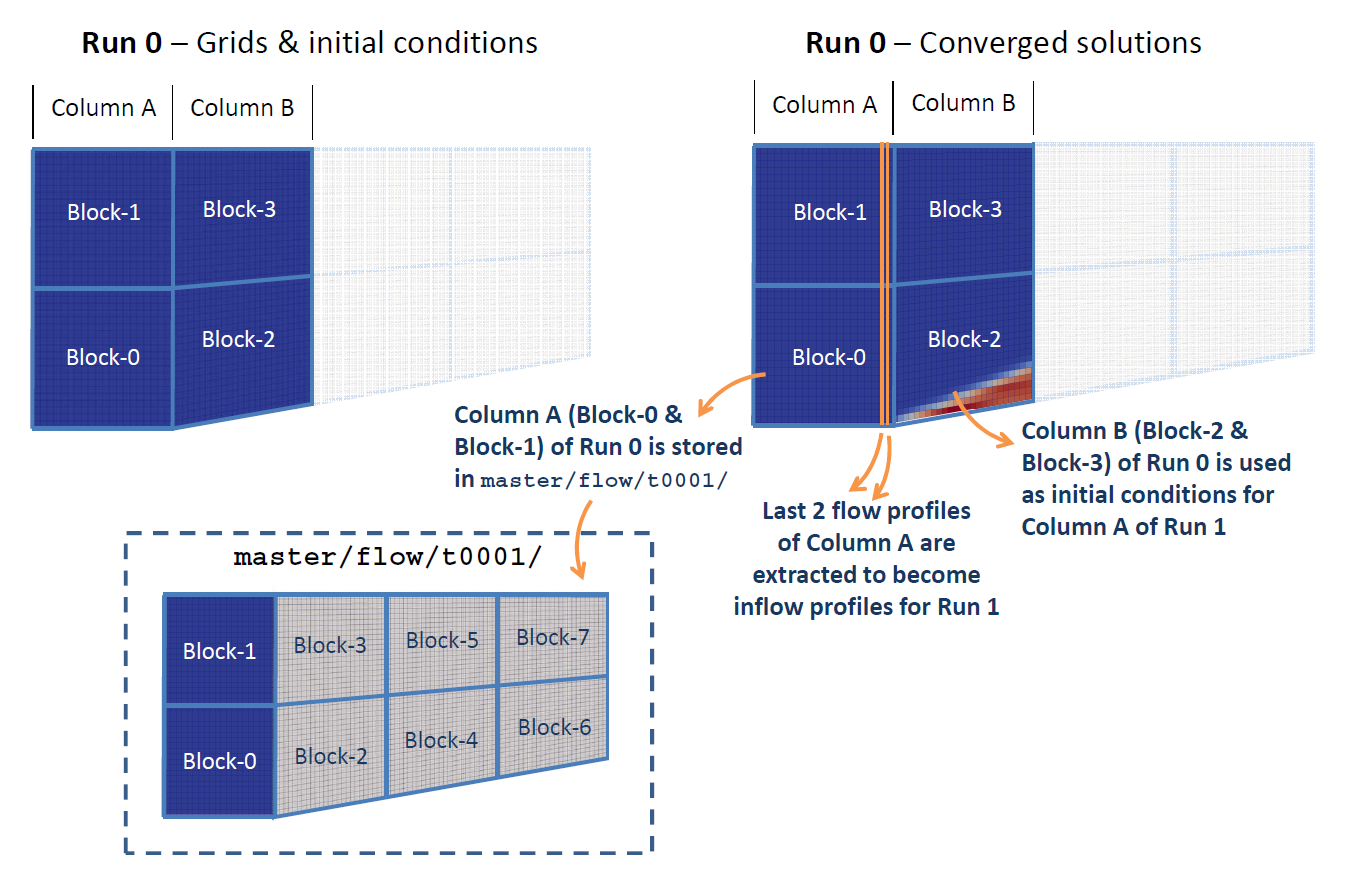
\includegraphics[width=15cm]{figs/e3march-run-0.png} }
   \caption{Run\,0 of the 10$^\circ$ wedge example.}
   \label{f:wedge10-run-0}
\end{figure}

\medskip
Run\,1 of the block-marching solver continues downstream by one column of blocks, 
as shown in Figure~\ref{f:wedge10-run-1}. Column\,A now consists of Block-2 and 
Block-3, while Column\,B consists of Block-4 and Block-5. For this run, the inflow
comprises of the two flow profiles extracted from the previous run. The initial
conditions for Column\,A are the converged solutions from the previous run, while
the initial conditions for Column\,B are built by propagating the flow properties
in the most downstream vertical slice of cells in Column\,A to all vertical slices
in Column\,B, as shown in the left diagram of Figure~\ref{f:wedge10-run-1}. The 
initial conditions for Column\,B are generated in this manner to help the simulation 
achieve a faster convergence to the steady-state solution. Upon the completion of 
Run\,1, the converged solutions are treated in the same manner as that for the 
converged solutions in Run\,0, as shown in Figure~\ref{f:wedge10-run-1}.
%
\begin{figure}
   \centerline{ 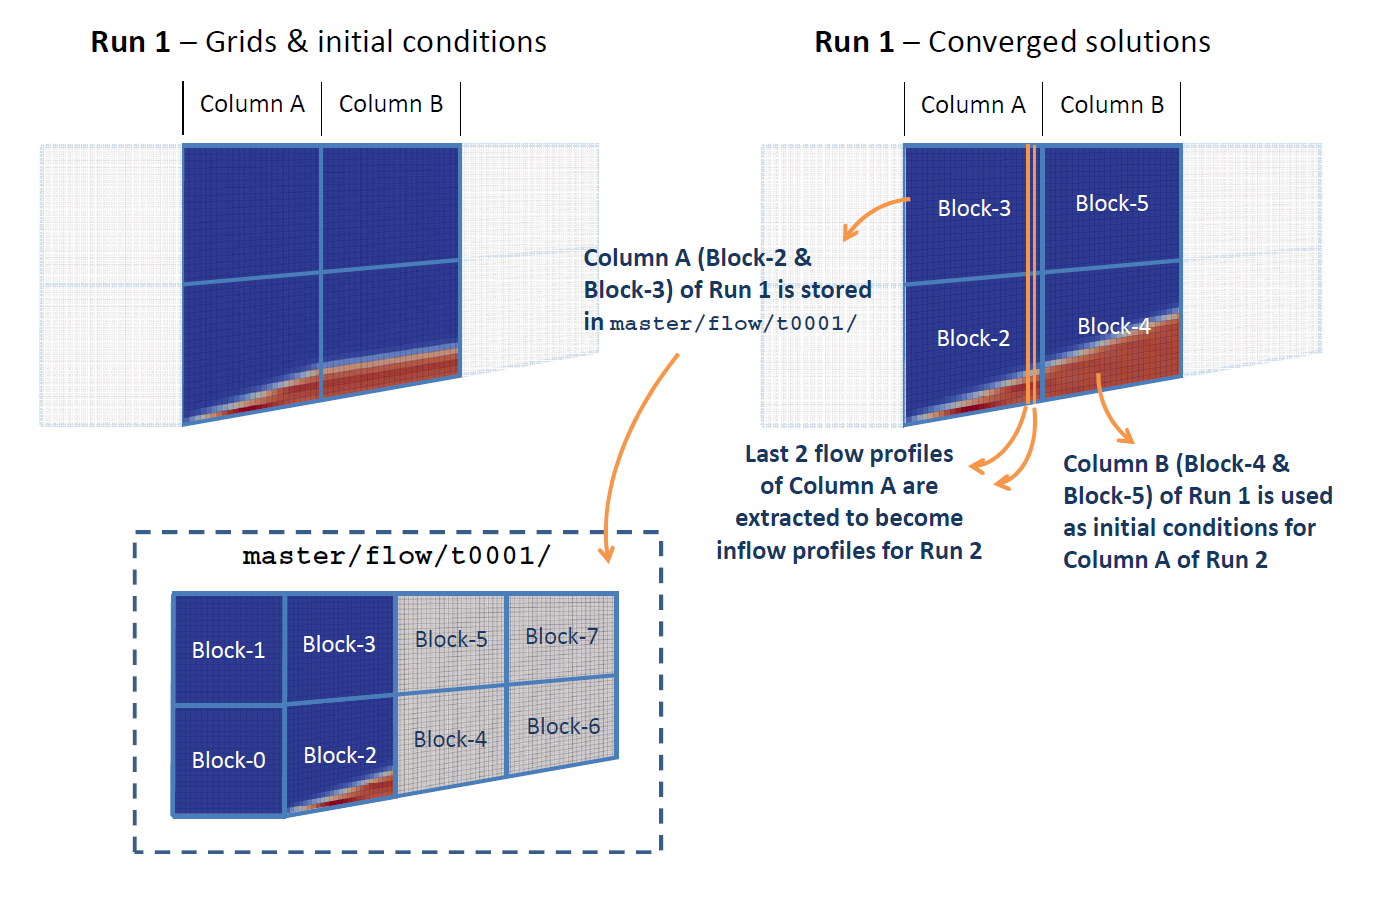
\includegraphics[width=16cm]{figs/e3march-run-1.png} }
   \caption{Run\,1 of the 10$^\circ$ wedge example.}
   \label{f:wedge10-run-1}
\end{figure}
%
\begin{figure}
   \centerline{ 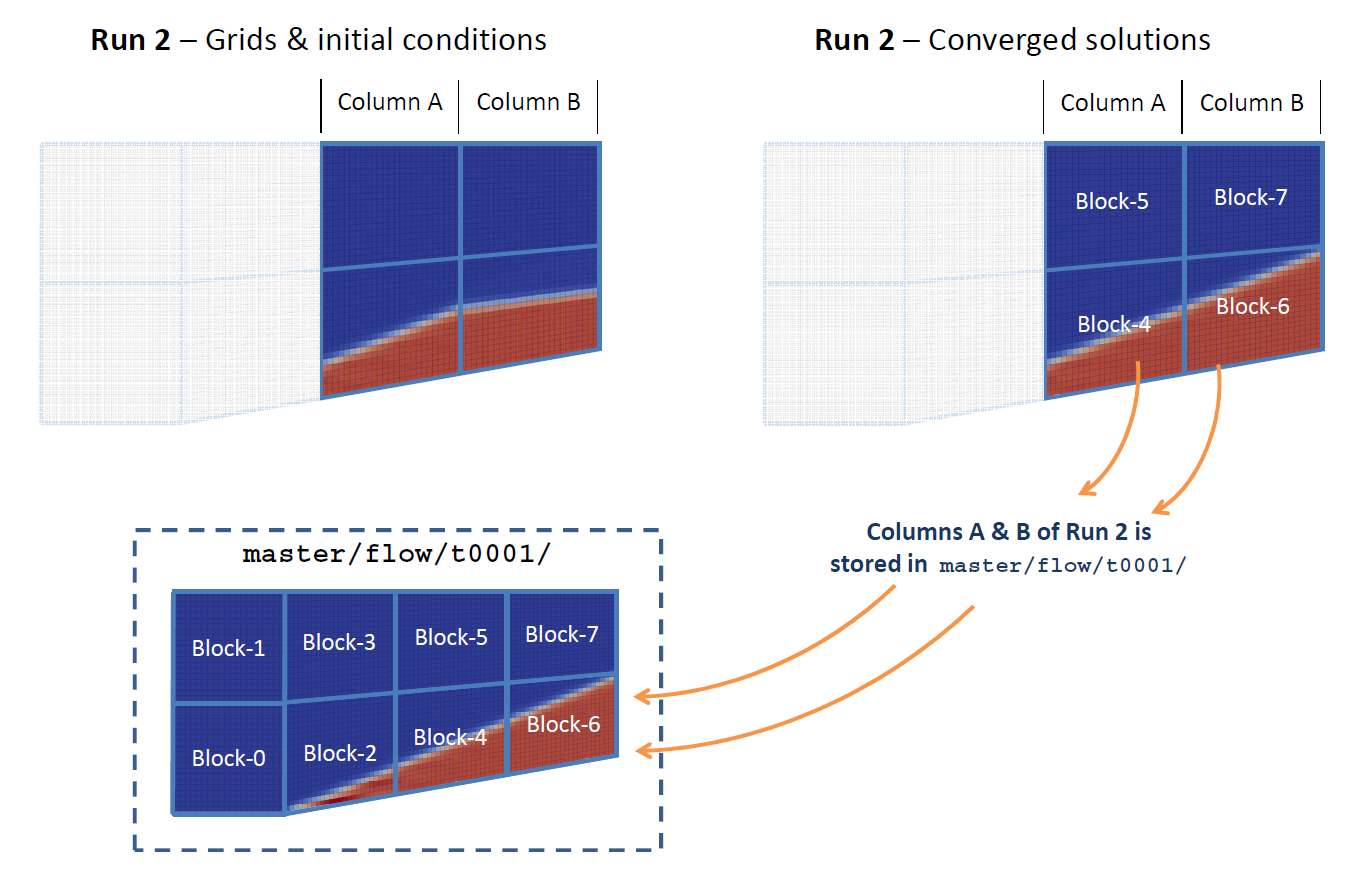
\includegraphics[width=16cm]{figs/e3march-run-2.png} }
   \caption{Run\,2 of the 10$^\circ$ wedge example.}
   \label{f:wedge10-run-2}
\end{figure}

\medskip
These steps are then repeated for Run\,2, as shown in Figure~\ref{f:wedge10-run-2}.
Since there are no remaining blocks to solve, this is the final run of the block-marching
process for this example. When Run\,2 is completed, the last two columns of data are 
stored in the \texttt{master/flow/t0001} folder, as shown 
in Figure~\ref{f:wedge10-run-2}. The block-marching process is then completed with the
transfer of all files in the \texttt{master} folder to the original working directory
and the deletion of any files that have been generated as a result of the block-marching
process.

\medskip
For each local run of the block-marching process, the run time is that for the global 
simulation divided by the number of local runs. In addition, the final time step for 
each local run is used as the initial time step for the next run to help achieve 
faster convergence to the steady-state solution.


\clearpage
\section{Examples}

\subsection{Channel with circular-arc bump}
%
Classic case for testing inviscid solvers.  
Sudden changes at start and end of bump set off oblique shocks that propagate across blocks..


\subsection{Reacting flow in a supersonic streamtube}
%
From Fabs' report.  
We have to get our chemistry right...


\subsection{Laminar boundary layer on a flat plate}
%
Comparison with Shetz boundary-layer code.


\subsection{Turbulent boundary layer on a flat plate}
%
Coles flat plate, maybe.


\subsection{Mohammadian convex plate}
%
Laminar boundary layer with pressure gradient.


\subsection{Glancing shock interaction with a boundary layer}
%
3D case


\clearpage
\bibliographystyle{unsrt}
\bibliography{bibtex/pj,bibtex/computing,bibtex/gas_dynamic,bibtex/adm,bibtex/gas,bibtex/dan,bibtex/upwind,bibtex/wilson}

\clearpage
\appendix
\section{Source code}

\noindent
\code{}{../../../app/eilmer3/source/e3march.py}

\clearpage
\phantomsection % re-set the hyperref anchor so that TOC page number link is correct.
\addcontentsline{toc}{part}{\indexname}
\printindex
\end{document}
